\chapter{Algae transport in a canal (canal\_algae)}

\section{Purpose}

This test case validates the algae transport module in \telemac{2D}, and it is a
useful example for a user wanting to see how to make use of the particle
positions and velocities.
%In addition, there is a Python script (\texttt{ConvertDat2Vtu.py}), added to
%this test case which can be used to convert the particle
%result file from a Tecplot format to a ParaView format.

In addition, there is a Python script
(\texttt{convert\_drogues\_file\_to\_vtuConvertDat2Vtu.py})
used in the \texttt{vnv\_canalalgae.py} validation script to convert the particle
result file from a Tecplot format to a ParaView format.

\section{Description}

To validate the algae bloom transport model, the experiment presented in
\citet{Joly2011} and \citet{Joly_jhr} is modelled.
More validation of the theory can also be found in \citet{Joly_pof}.
The flow configuration of this experiment is that of partially obstructed open
flat bed channel flow, which has the advantage of generating a large
recirculation pattern downstream of the obstructing groyne.
In this experiment a fluid with a density of 1,000~kg/m$^3$ and a flow rate of
0.5~m/s is imposed in a 2~m wide channel which is obstructed by a groyne 0.5~m
long and 0.1~m thick.
The water depth is imposed to be 0.3~m before the flow arrives at the groyne.
The groyne is constructed high enough to stop overtopping.
The experimental setup is described in Figure~\ref{fig:exp_setup}, and the
Reynolds number is thus 10$^6$.

\begin{figure}[hb]
\begin{center}
  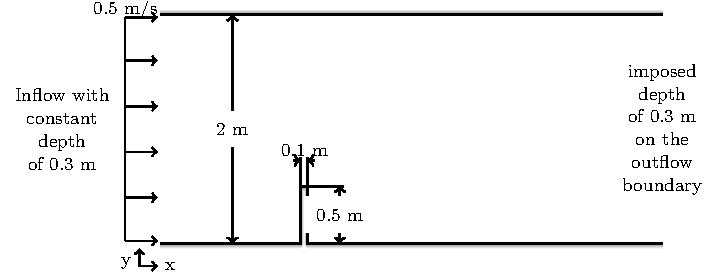
\includegraphics[width=0.75\textwidth]{./img/CanalAlgExpSetup}
\end{center}
\caption{Experimental setup for a partially obstructed flat bed open channel flow (top view). In this experminent
spherical particles are released to validate the algae transport of \telemac{2D}.}
\label{fig:exp_setup}
\end{figure}

The flow velocities are well modelled using \telemac{2D}.
In this case, the flow is modelled using a $k$-$\varepsilon$ closure and it is
validated against experimental measurements and another simulation performed
with OpenFoam, which solves the two-dimensional Navier-Stokes equations with a
$k-\varepsilon$ closure using a finite volumes method.
The horizontal fluid velocities are presented in
Figure~\ref{fig:profil_vitesses_canal}.

\begin{figure}[H]
\begin{center}
  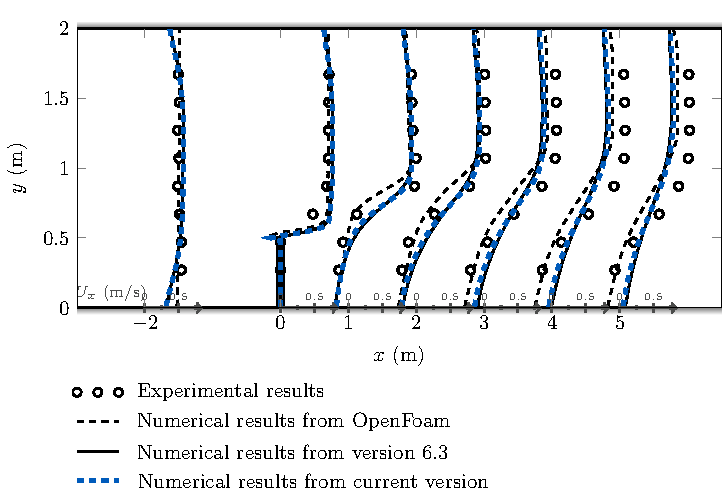
\includegraphics[width=0.75\textwidth]{./img/CanalAlgFluidVelocities}
\end{center}
\caption{Profiles of the horizontal velocity plotted at different locations along the canal. The small axis marked on
top of the $x$-axis represent the values of velocity magnitude.}
\label{fig:profil_vitesses_canal}
\end{figure}

Spheres 6~mm in diameter ($D_s$) and of density $\rho_s$ = 2,200~kg.m$^{-3}$
are released in the flow one at a time at fixed intervals (about 1~Hz).
This is done to ensure that particles would not affect each other's motion.
Several particles are released at different positions in the flow and the
trajectories for these particles are recorded at different locations.
The trajectories of these particles are measured with a camera that is placed
above the flow so that the position of particles entering a window of measurement
are recorded, see Figure~\ref{fig:exp_setup2}.
The process used to extract the trajectories is presented in \citet{Joly2011}.

\begin{figure}[H]
\begin{center}
  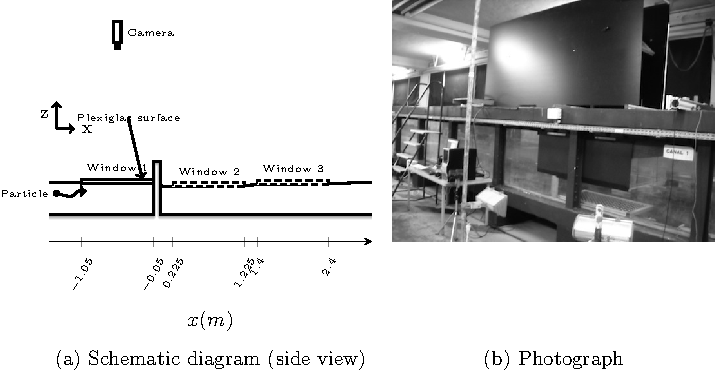
\includegraphics[]{./img/CanalAlgExpSetup2}
\end{center}
\caption{Experimental setup to record the particle trajectories.}
\label{fig:exp_setup2}
\end{figure}

\subsection{Geometry and mesh}

The mesh consists of the mesh has 36,996 nodes and 73,346 elements.
The mesh elements size is about 0.1~m at the inflow, 0.015~m around the groyne
and 0.3~m at the outflow.
A picture of the mesh can be found in Figure~\ref{fig:mesh_obstruc_channel}.

\begin{figure}[H]
\begin{center}
  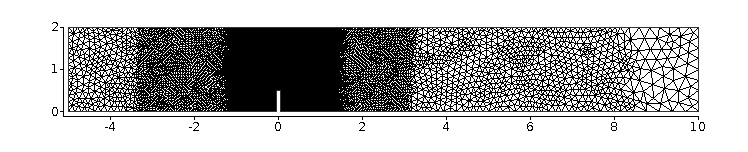
\includegraphics[width=0.85\linewidth]{./img/Images/mesh_obstruc_channel}
\end{center}
\caption{Mesh used to simulate the obstructed channel flow.}
\label{fig:mesh_obstruc_channel}
\end{figure}

\subsection{Numerical parameters}
To help the simulation run faster, the computation is continued from a previous
file, i.e. using the following keywords:

\lstset{language=TelemacCas,
        basicstyle=\scriptsize\ttfamily}

\begin{lstlisting}[frame=trBL]
COMPUTATION CONTINUED = YES
PREVIOUS COMPUTATION FILE =
'./ini_canal_algae_en.slf'
INITIAL TIME SET TO ZERO = YES
\end{lstlisting}

In the simulations 1,000 spheres will be released with diameter 0.006~m and
density 2,200~kg.m$^{-3}$.
The following keywords activate the algae transport module and set these
physical characteristics:

\lstset{language=TelemacCas,
        basicstyle=\scriptsize\ttfamily}

\begin{lstlisting}[frame=trBL]
/----------------------------------------------------------------------/
/                     ALGAE OPTIONS
/----------------------------------------------------------------------/
MAXIMUM NUMBER OF DROGUES = 1000
PRINTOUT PERIOD FOR DROGUES = 40
ASCII DROGUES FILE = './alg_pos.dat'
ALGAE TRANSPORT MODEL = YES
DIAMETER OF ALGAE = 0.006
DENSITY OF ALGAE = 2200.0
ALGAE TYPE = 1
\end{lstlisting}

Finally, the particle defined by editing the user subroutine
\telfile{USER\_FLOT}, and adding these lines of code:

%      IF(LT.EQ.ALGAE_START) THEN

\lstset{language=Fortran,
        basicstyle=\scriptsize\ttfamily}

\begin{lstlisting}[frame=trBL]
      IF(LT.EQ.0) THEN
        DO I=1,NFLOT_MAX
          CALL ADD_PARTICLE(0.175D0,0.45D0,0.D0,I,NFLOT,
     &                    NFLOT_MAX,XFLOT,YFLOT,YFLOT,TAGFLO,
     &                    SHPFLO,SHPFLO,ELTFLO,ELTFLO,MESH,1,
     &                    0.D0,0.D0,0.D0,0.D0,0,0)
        END DO
      ENDIF
\end{lstlisting}

\section{Results}

\subsection{Explanation of the results}

For this test case, the particles are released at position (0.175, 0.45) and
recorded using window 2 (see \figurename~\ref{fig:exp_setup2}a).
More results are presented in \citet{Joly2011}.

To analyse the trajectories of the particles, the window of measurements is then
divided into four quadrants.
The number of particles entering each quadrant, and the time spent inside is
recorded.
The values are then non-dimensionnalised using the sum of all the quadrants, i.e.:

\begin{subequations}
\begin{align}
N_{res,Q_i}=&\frac{N_{Q_i}}{\sum_j^4{N_{Q_j}}},
\\
T_{res,Q_i}=&\frac{T_{Q_i}/\sum_j^4{T_{Q_j}}}{N_{Q_i}/\sum_j^4{N_{Q_j}}},
\end{align}
\end{subequations}

Where $N_{res,Q_i}$ and $T_{res,Q_i}$ represent the non-dimensionnalised
proportion of particles and mean time of residence inside a quadrant
$Q_i$. $N_{Q_i}$ is the number of particles recorded in a quadrant and $T_{Q_i}$
is the cumulative time spend by all the particles present in this quadrant.

This method of writing the results allows a comparison between numerical and
experimental results, as during the experiment it is impossible to know if a
particle that exited the window of measurement would re-enter it at a later time.

These results are plotted in Figures~\ref{fig:quadrant_npart}
and~\ref{fig:quadrant_tresid}, where for each quadrant the value of interest is
plotted along a line going from the inner most corner to the outter most corner.
The length scales for these values are chosen in such a way that the maximum
value is placed on the outer most corner.
The points plotted for each quadrant are then linked together to form an area.
An annotated description of the results is given in
\figurename~\ref{fig:expe_canal_annotated_example}.

\begin{figure}[H]
\begin{center}
  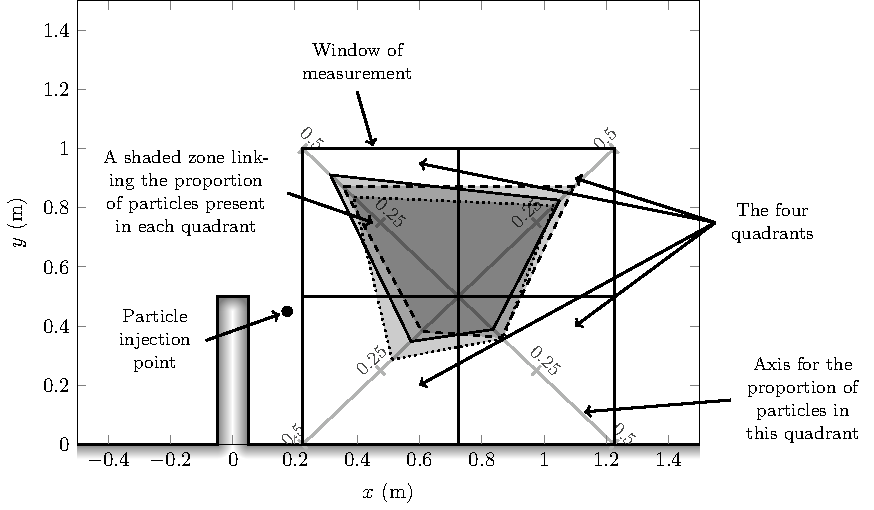
\includegraphics[]{./img/CanalAlgAnnotatedFigure}
\end{center}
\caption
{An annotated example to explain how the proportion of particles entering each quadrant of a window of measurement are presented.}
\label{fig:expe_canal_annotated_example}
\end{figure}

The velocities of the particles are also analysed.
To do so, profile plots are done of the properties of the particles crossing
the line at $x$ = 0.55~m.
These figures can be found in Figures~\ref{fig:profile_x0p55_N}
to~\ref{fig:profile_x0p55_V_Y}.

\subsection{Simulation results}

The first result presented will be the proportion of particles entering a
quadrant and their mean time of residence.
These results will be compared to experimental results and results where the
fluid velocities are simulated using OpenFoam.
They are presented in
\figurename{}s~\ref{fig:quadrant_npart} and~\ref{fig:quadrant_tresid}.

\begin{figure}[H]
\begin{center}
  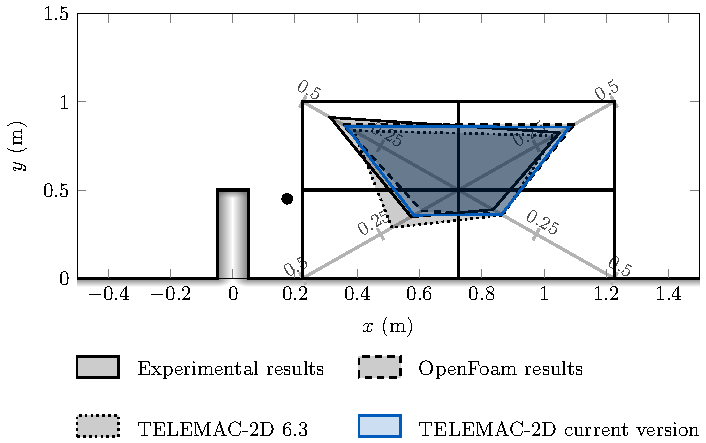
\includegraphics[]{./img/CanalAlgQuadrantNpart}
\end{center}
\caption{Partially obstructed channel flow: proportion of released particles entering a quadrant of the window of measurement.}
\label{fig:quadrant_npart}
\end{figure}

\begin{figure}[H]
\begin{center}
  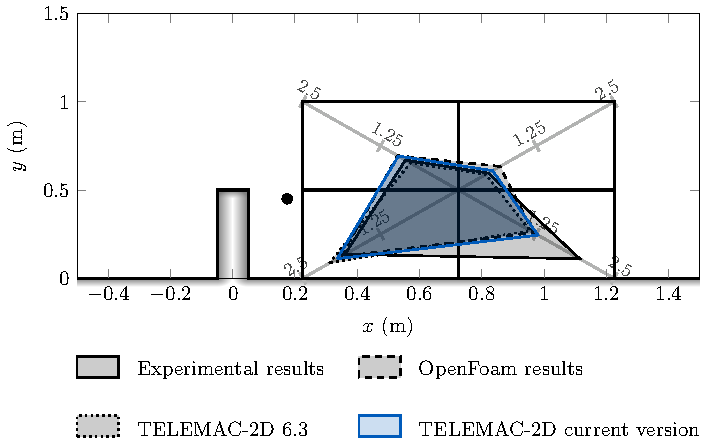
\includegraphics[]{./img/CanalAlgQuadrantTrsd}
\end{center}
\caption{Partially obstructed channel flow: mean particles residence time inside a quadrant of the window of measurement.}
\label{fig:quadrant_tresid}
\end{figure}

As can be seen from \figurename{}s~\ref{fig:quadrant_npart}
and~\ref{fig:quadrant_tresid}, the \telfile{ALGAE\_TRANSP} module
models accurately the position of spherical particles.
There is only the mean time of residence of the bottom right corner which has
noticeable differences, but this is also the case with the fluid velocities
model using OpenFoam.
This would suggest that the center of the recirculation pattern might be a bit
off when modelled in \telemac{2D}.

The next results will assess the ability of the model to predict the velocities
of the particles released in the flow.
In \figurename{}s~\ref{fig:profile_x0p55_N} to~\ref{fig:profile_x0p55_V_Y}
profiles will be shown of the fraction of particles crossing the section defined
by $x$ = 0.55~m, as well as the horizontal and vertical velocities ($V_x$ and $V_y$).

\begin{figure}[h!]
\begin{center}
  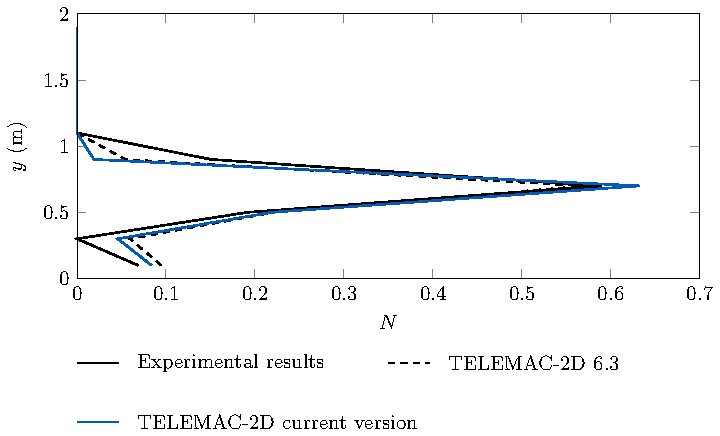
\includegraphics[]{./img/CanalAlgProfile_x0p55_N}
\end{center}
\caption{Partially obstructed channel flow: fraction of particles crossing the section defined by $x$ = 0.55~m.}
\label{fig:profile_x0p55_N}
\end{figure}

\begin{figure}[h!]
\begin{center}
  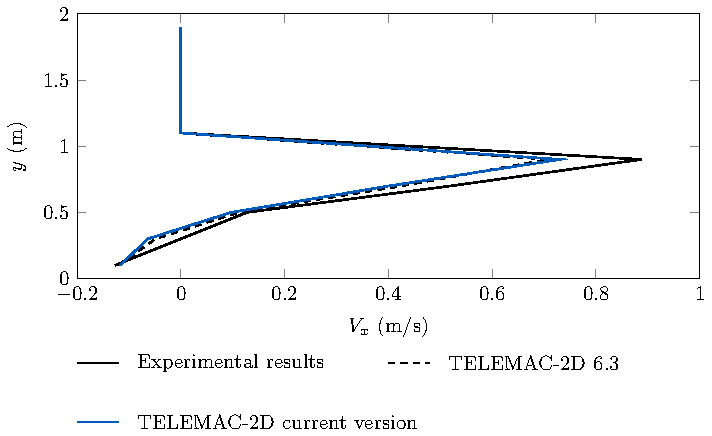
\includegraphics[]{./img/CanalAlgProfile_x0p55_Vx}
\end{center}
\caption{Partially obstructed channel flow: velocity along $x$-axis of particles crossing the section defined by $x$ = 0.55~m.}
\label{fig:profile_x0p55_V_X}
\end{figure}

\begin{figure}[h!]
\begin{center}
  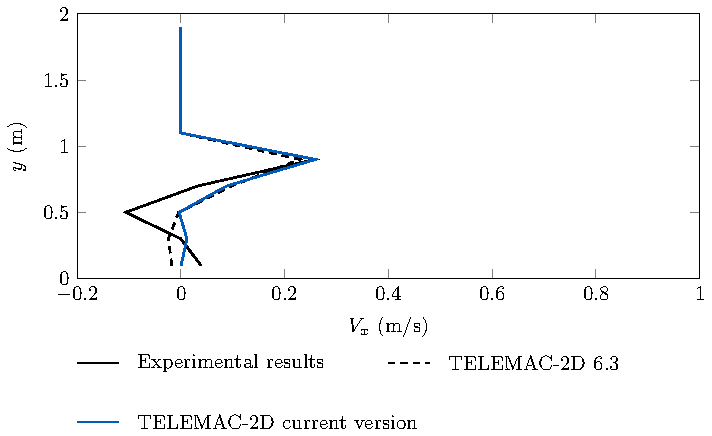
\includegraphics[]{./img/CanalAlgProfile_x0p55_Vy}
\end{center}
\caption
{Partially obstructed channel flow: velocity along $y$-axis of particles crossing the section defined by $x$ = 0.55~m.}
\label{fig:profile_x0p55_V_Y}
\end{figure}

The results presented in Figures~\ref{fig:profile_x0p55_N}
to~\ref{fig:profile_x0p55_V_Y} show again that the module \telfile{ALGAE\_TRANSP}
models accurately the velocity.
The only region of error would be for the vertical velocity near the solid
boundaries, but this is probably linked to the previous mis-estimation of the
center of the recirculation pattern in \telemac{2D}.
Furthermore the results are still independent of the number of processors used.

\chapter{Algae transport in a canal 2 (canal\_algae)}

\section{Purpose}

The purpose of this example is to show that the initial algae distribution for a
test with algae can be defined in a number of different ways.

\section{Description of the test case}

This test case is based on the \textbf{canal\_algae} test case.
The only difference is the initial distribution of the algae.
The details of the model can be found in the description for Algae Canal.

\begin{figure}[h]
  \begin{center}
    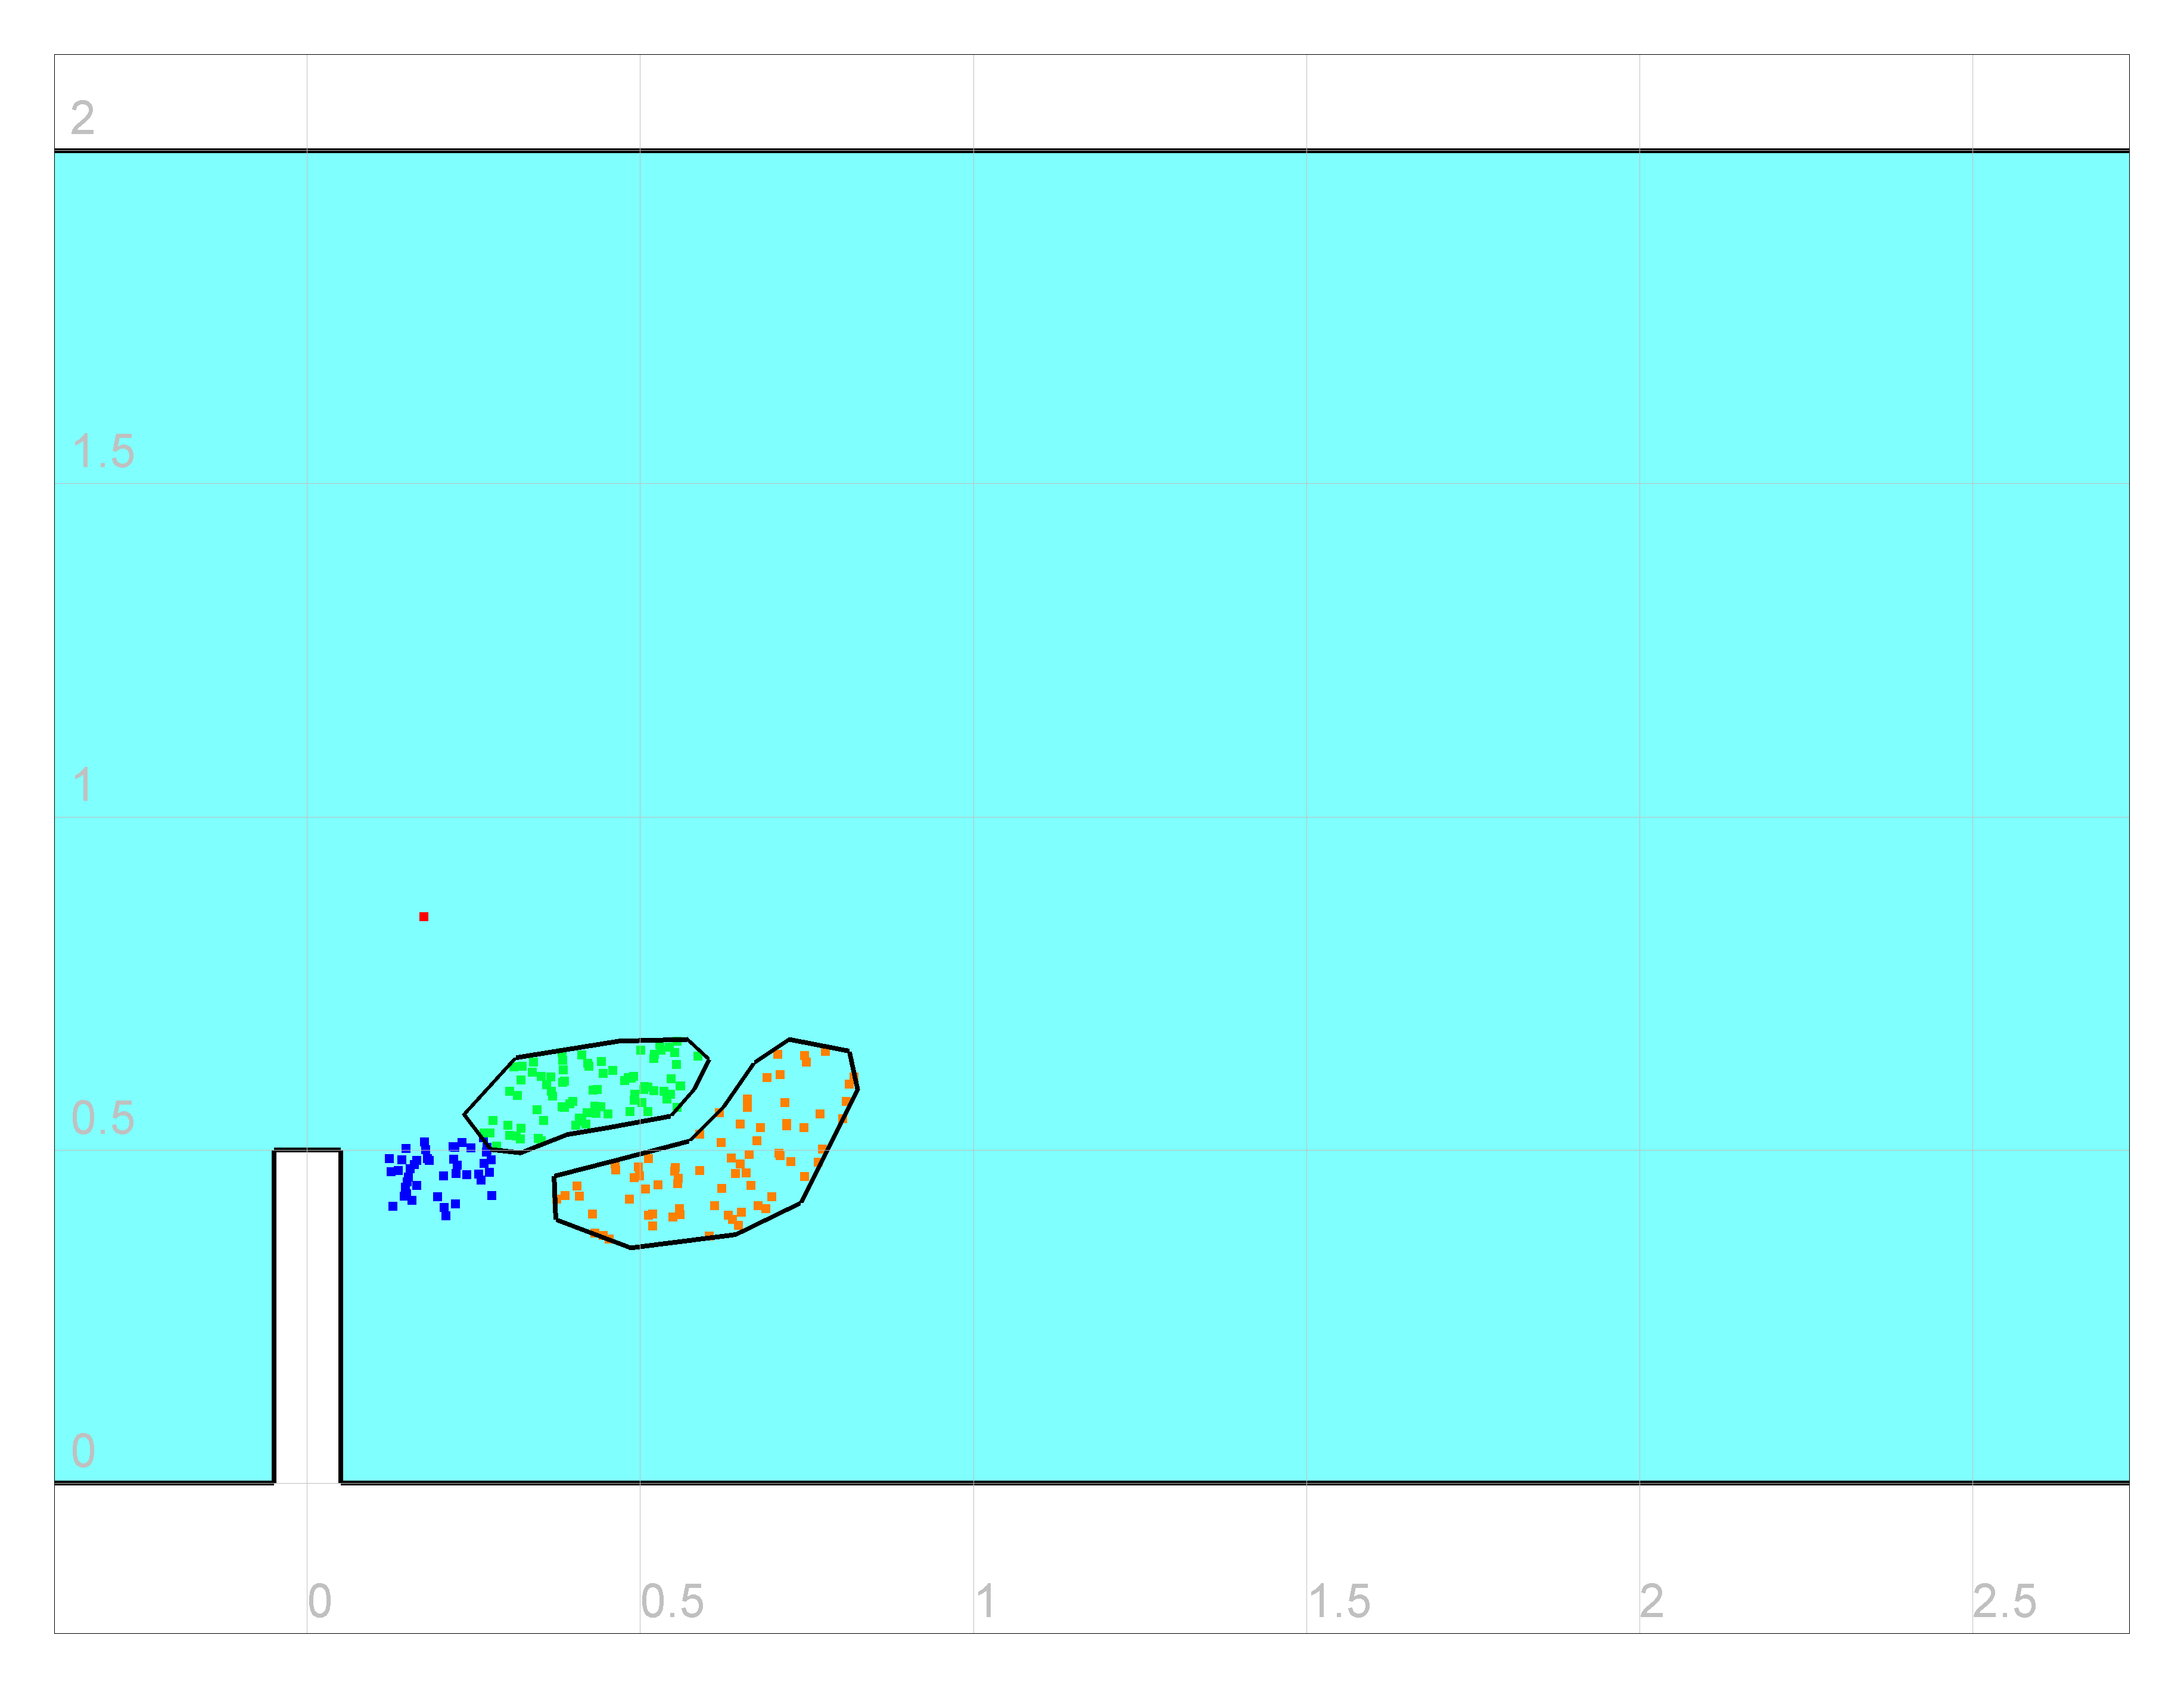
\includegraphics[width=0.75\textwidth]{./img/canal_algae_initial_02}
  \end{center}
  \caption{Initial algae distribution.}
  \label{fig:exp_init}
\end{figure}

There are 500 algae particles at $x$ = 0.175~m, $y$ = 0.45~m.
These are defined in the subroutine \telfile{USER\_FLOT}, which uses the
subroutine \telfile{ADD\_PARTICLE} to add each algae particle.
These are defined with class 4.

\smallskip
A second group of particles is defined using a polygon file, containing two
polygons, which is specified using the keyword
\telkey{DROGUES INITIAL POSITIONING DATA FILE}.
The polygon file must be in the Blue Kenue i2s format.
These two polygons are shown in Figure~\ref{fig:exp_init}.
The left polygon has defined some particles of class 2.
The right polygon has defined some particles of class 3.

\smallskip
A third group of particles is defined using a variable called
\telfile{DROGUES CLASSES} in the geometry file.
In this case, there is an area close to the groyne where this variable is equal
to 1.
Elsewhere the variable is zero.
This has resulted in a region of algae particles close to the groyne with class 1.

\smallskip
The keyword \telkey{INITIAL DROGUES SAMPLING DENSITY} gives the number of algae
particles per unit area for a given class, for the cases where the algae is
defined by polygons or the geometry file.
In this case, the density is 2,000 for class 1 and class 2 particles and 1,000
for class 3 particles. 

Figure~\ref{fig:exp_init} plots algae particles with class 1 as blue, class 2 as
green, class 3 as orange and class 4 as red.

\smallskip
The keyword \telkey{DURATION BEFORE ALGAE RELEASE} gives the time of release (in
seconds) for a given class.
In this case the release times are 5~s for class 1, 10~s for class 2, 15~s for
class 3 and 0~s for class 4.

\section{Results}

The algae distribution after 3 seconds, 12 seconds and 30 seconds (the end of
the run) is shown in Figure~\ref{fig:res_3s} to Figure~\ref{fig:res_30s}.
By 30 seconds, most of the particles have left the domain through the right
boundary.

\emph{Because of the randomisation of the turbulent particle movements the
  result on the reader's machine may be slightly different to the results below, but it should be similar.}

\begin{figure}[h]
  \begin{center}
    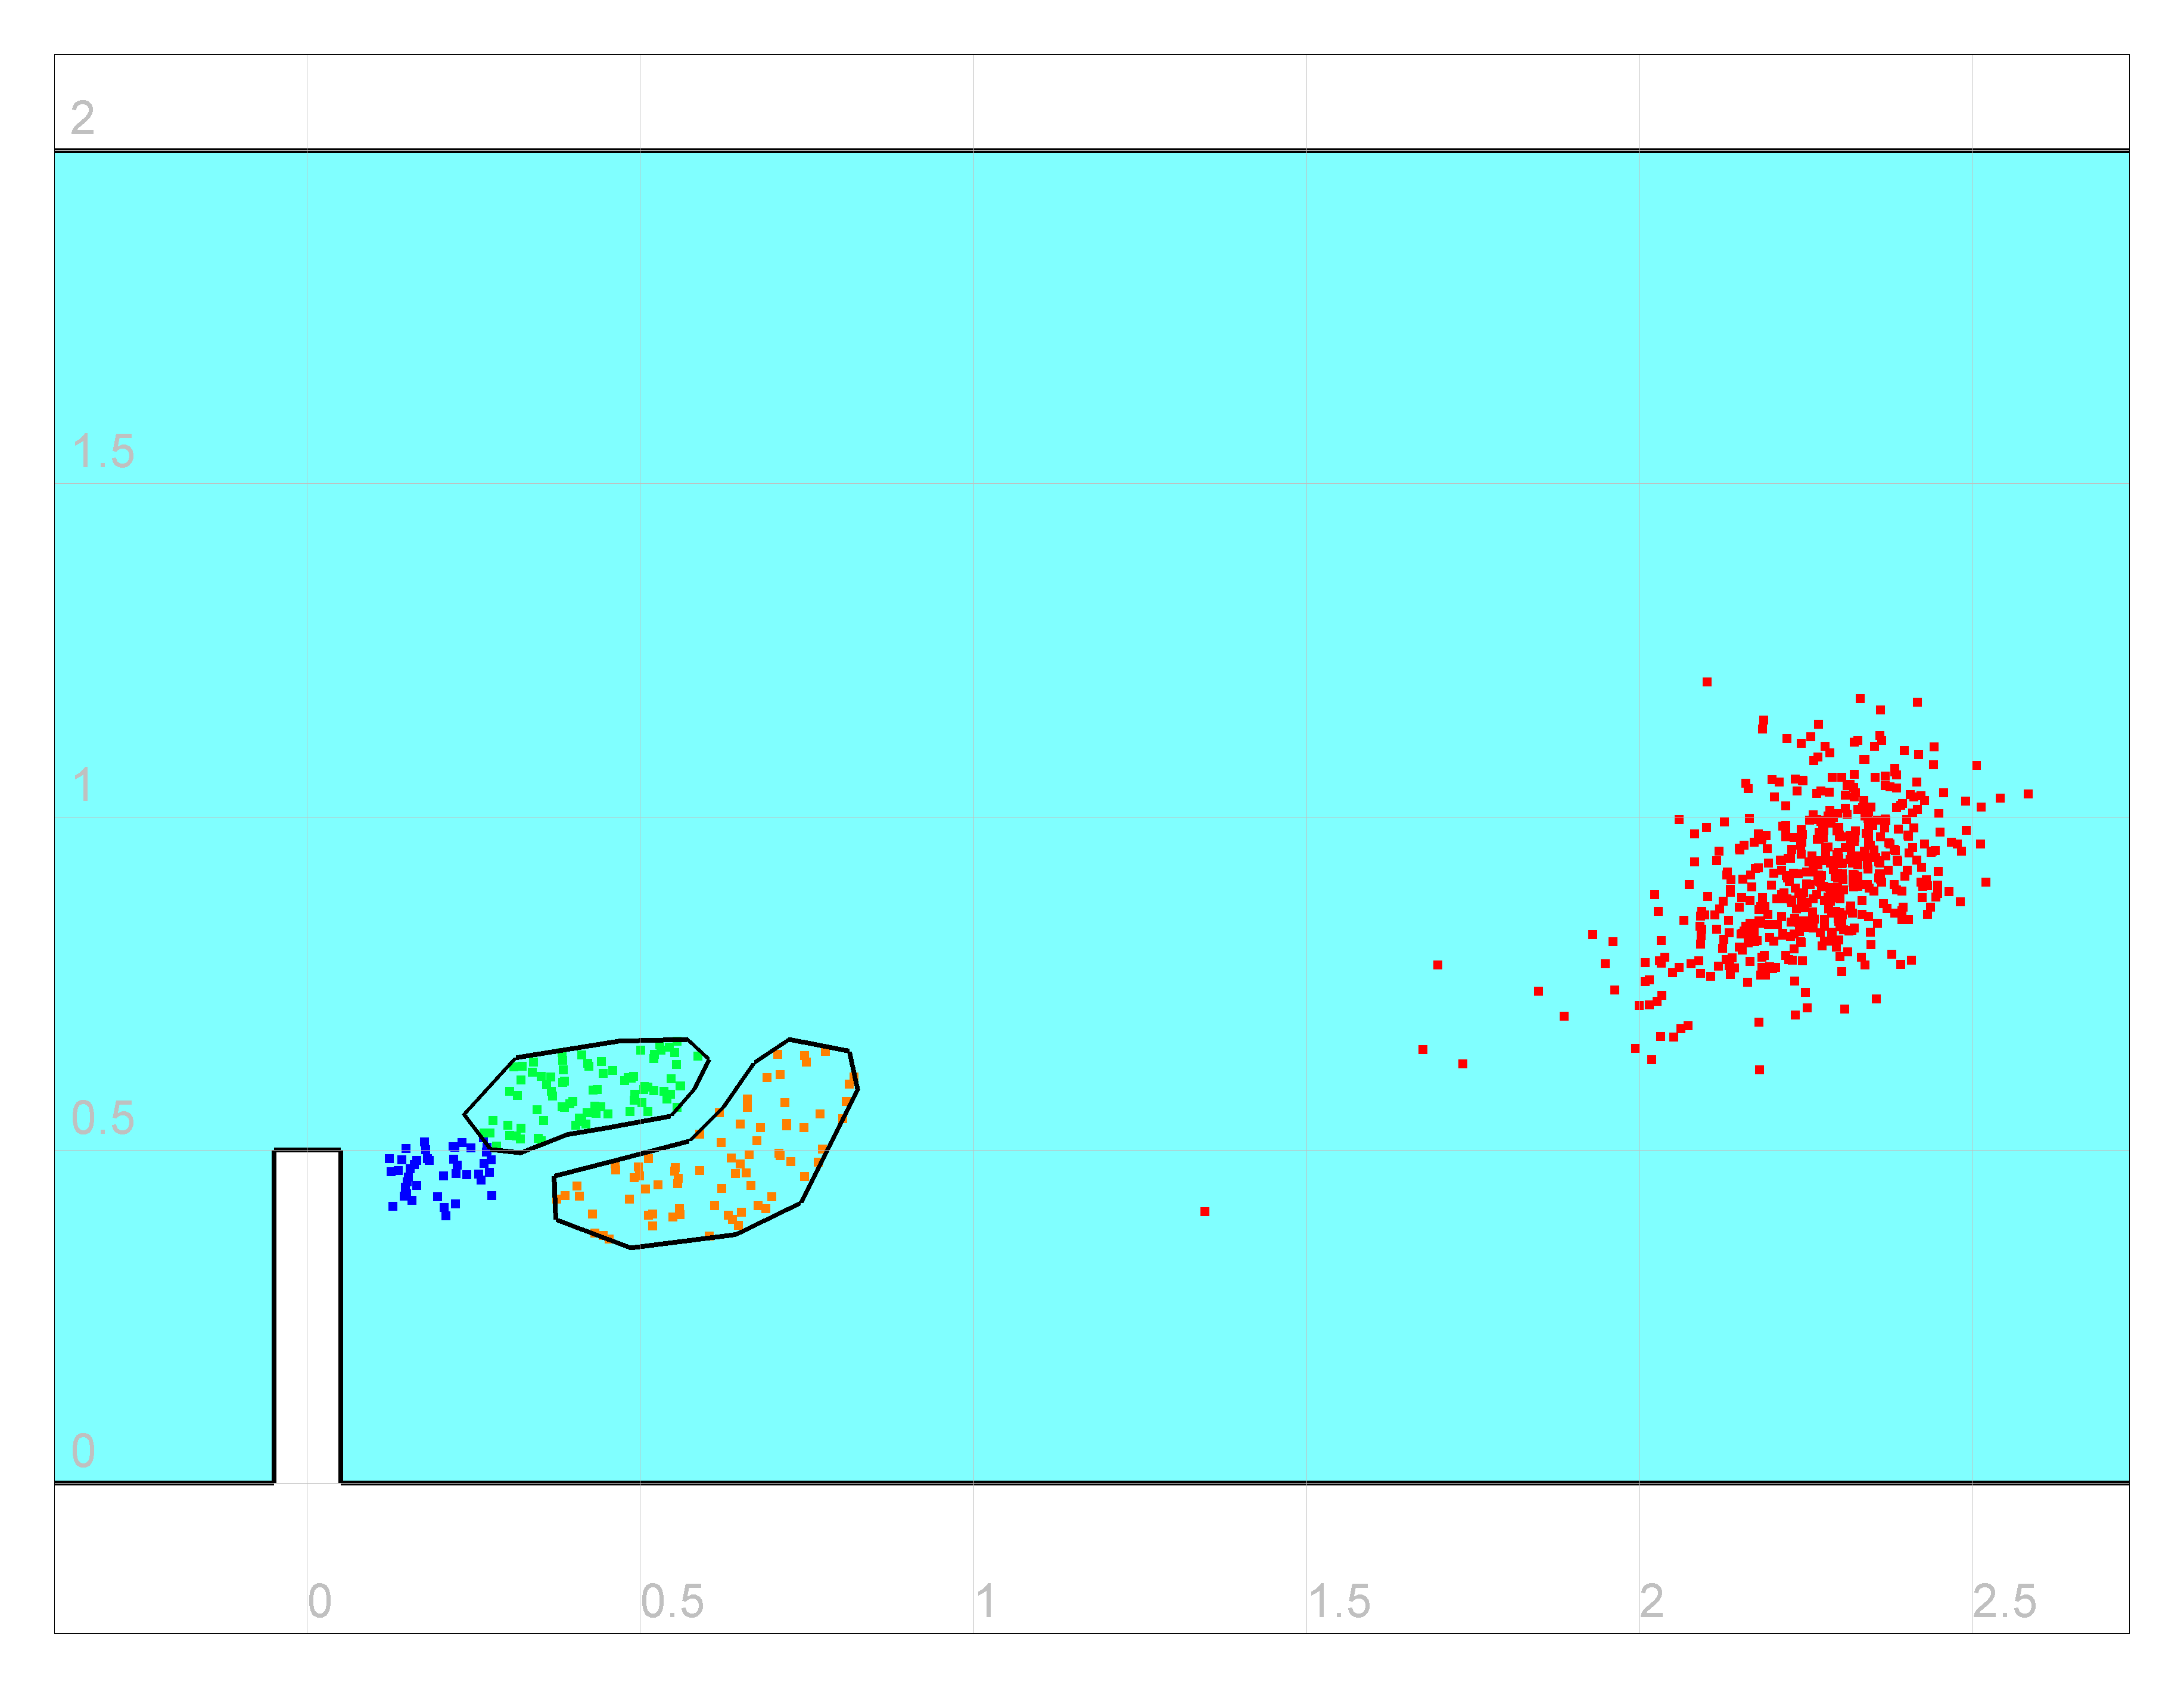
\includegraphics[width=0.75\textwidth]{./img/canal_algae_3s_02}
  \end{center}
  \caption{Algae distribution after 3~s.}
  \label{fig:res_3s}
\end{figure}

\begin{figure}[h]
  \begin{center}
    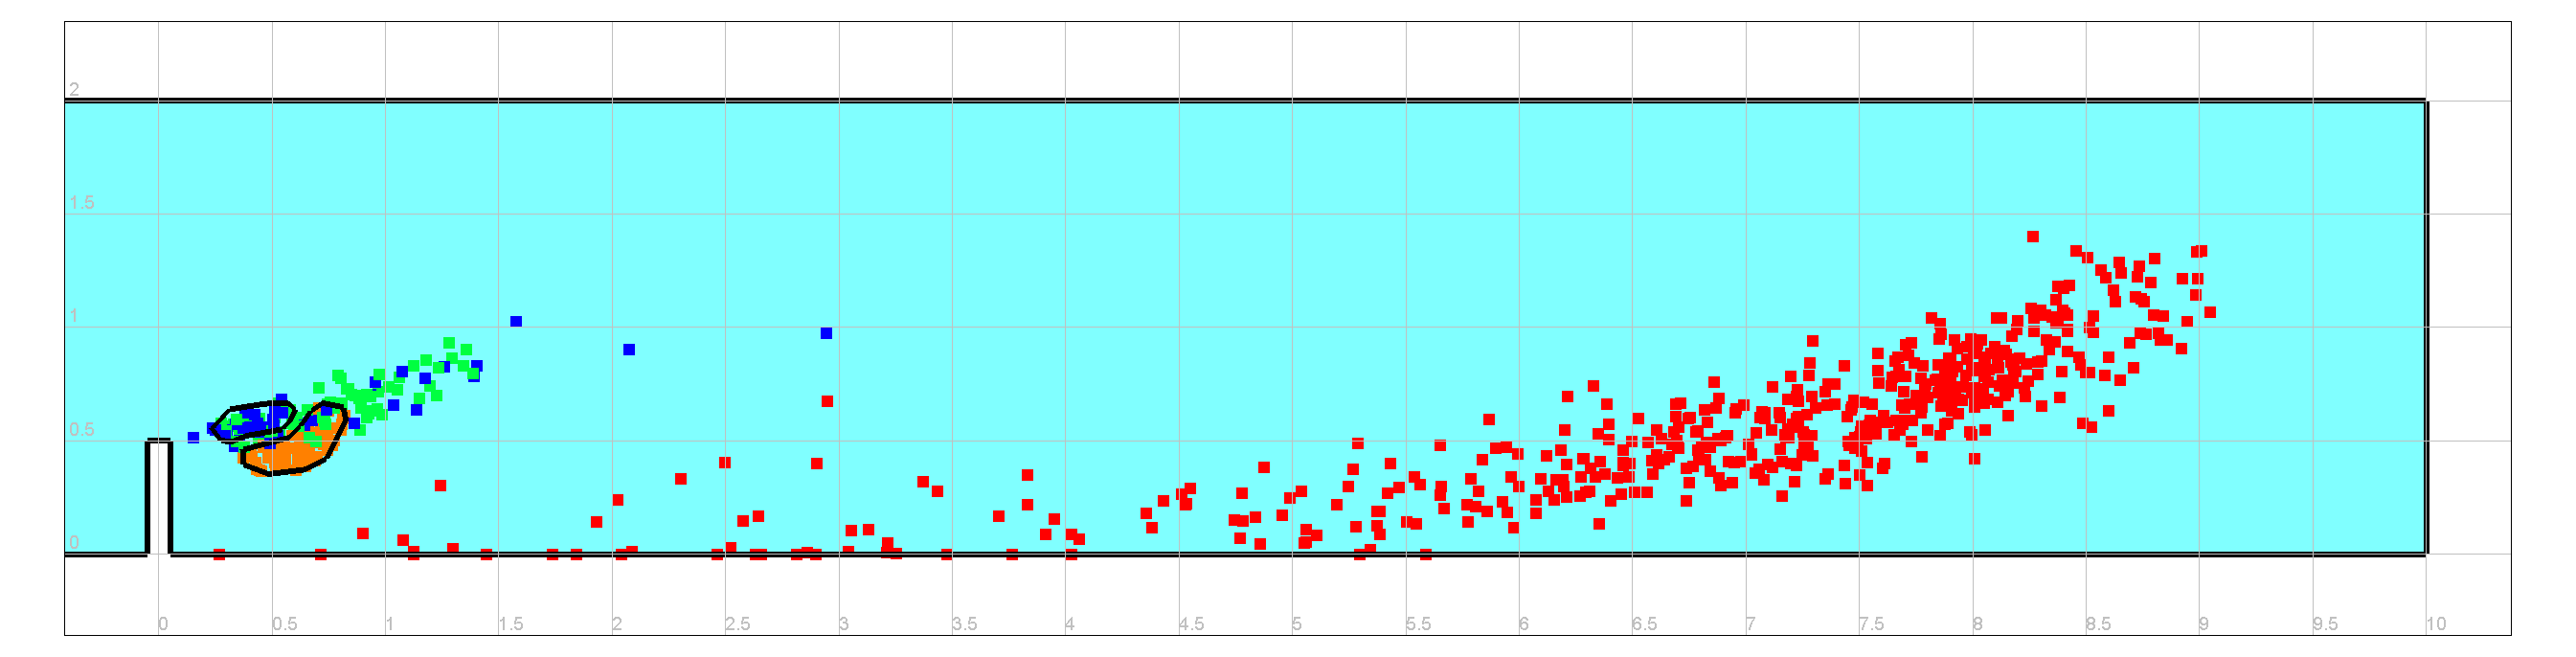
\includegraphics[width=0.75\textwidth]{./img/canal_algae_12s_02}
  \end{center}
  \caption{Algae distribution after 12~s.}
  \label{fig:res_12s}
\end{figure}

\begin{figure}[h]
  \begin{center}
    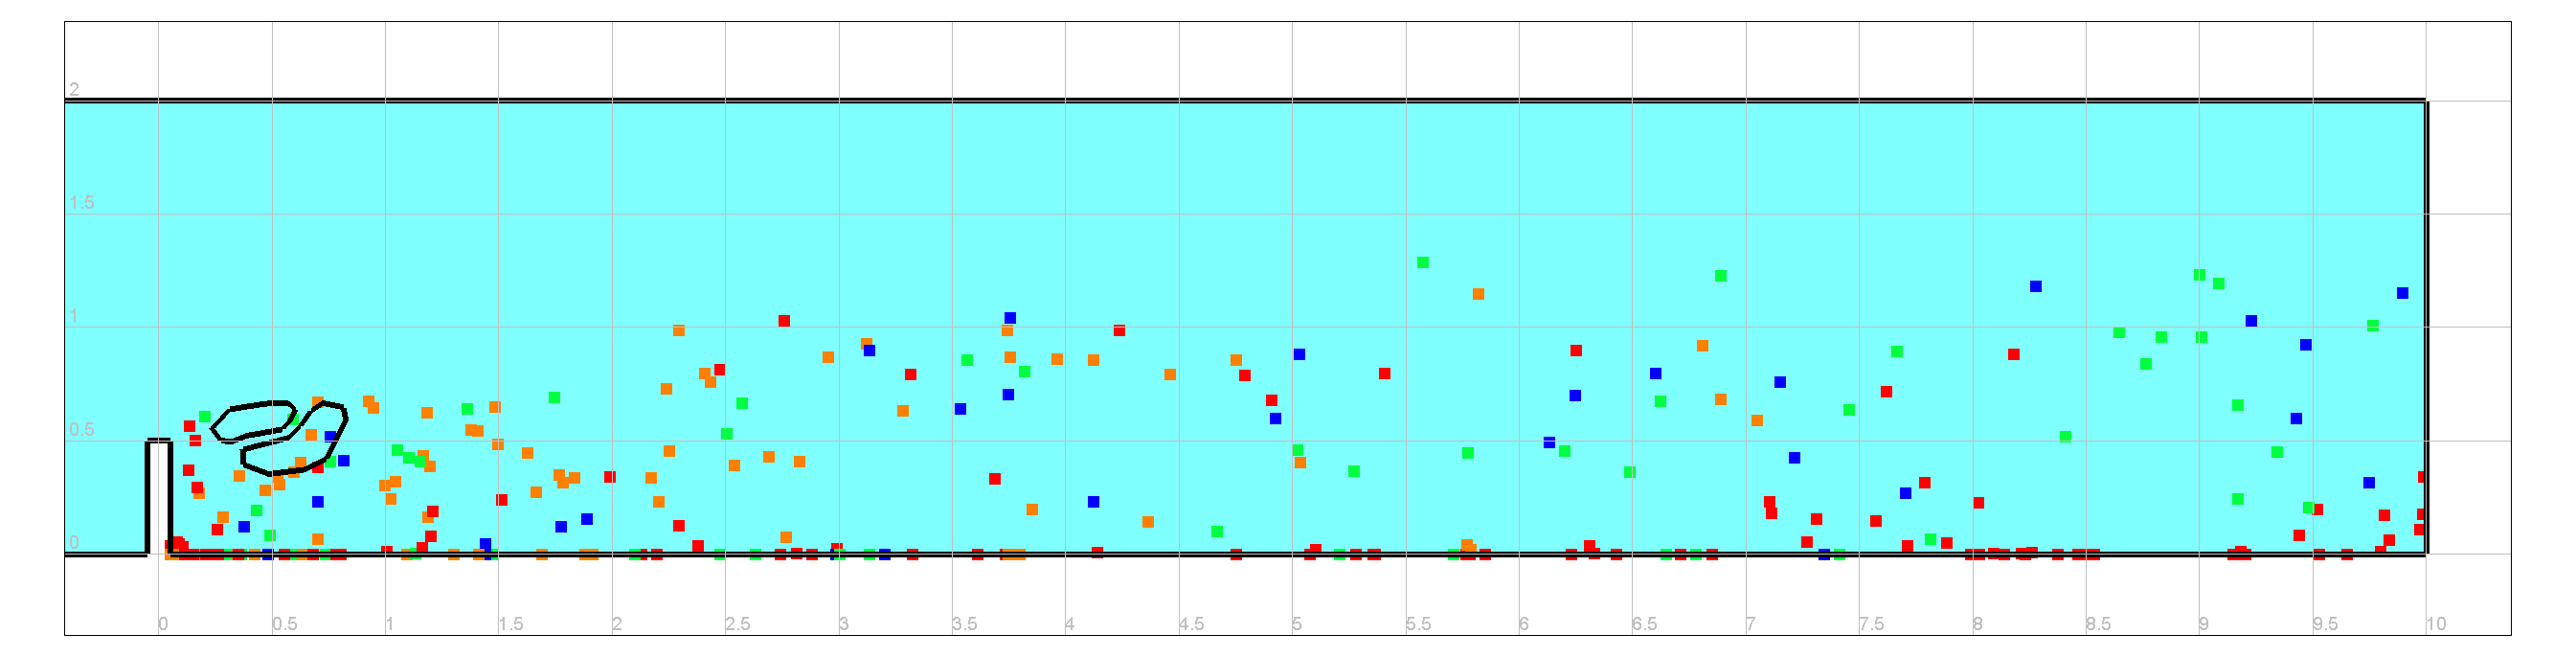
\includegraphics[width=0.75\textwidth]{./img/canal_algae_30s_02}
  \end{center}
  \caption{Algae distribution after 30~s.}
  \label{fig:res_30s}
\end{figure}

The standard test case outputs the algae information as a Tecplot file.
In this case, the algae information is written to a file defined by the keyword
\telkey{ASCII DROGUES FILE}.
The default value of the \telkey{DROGUES FILE FORMAT} is TECPLOT.
In order to output to a PCL file, give the output file name using the keyword
\telkey{BINARY DROGUES FILE} and give the \telkey{DROGUES FILE FORMAT} as BKBINPCL.
PCL files can be displayed using Blue Kenue.

\smallskip
This example outputs a text file called \verb!polygon_particles.txt!.
Output is written to the file every 0.1~s.
The output relates to four polygons that surround the four initial regions of
particles, as described above.
The first polygon surrounds the particles defined by the geometry file.
Polygons 2 and 3 are illustrated in the previous figures.
The fourth polygon surrounds the point with the initial 500 particles.
For each time, the output file contains the time, and the number of initial
particles that remain in the polygon and un-mobilised.    
Running of the test case should result in a text file identical to the
\verb!polygon_particles.txt! file.

\smallskip
For this test case example the random distribution of initial particles is fixed
through lines 39 to 47 of the \telfile{CONDIN\_DROGUES} subroutine.
These lines ensure that the particles are initially located in the same place
whenever the test case is run but should be commented out when running the code
more generally.  
